\documentclass[12pt,a4paper]{article}

\usepackage[utf8]{inputenc}
\usepackage[T1]{fontenc}
\usepackage[brazil]{babel}
\usepackage{geometry}
\usepackage{graphicx}
\usepackage{booktabs}
\usepackage{longtable}
\usepackage{array}
\usepackage{float}
\usepackage{hyperref}
\usepackage{xcolor}

\geometry{margin=2.5cm}
\setlength{\parindent}{0pt}
\setlength{\parskip}{0.65em}
\renewcommand{\arraystretch}{1.15}

\hypersetup{
    colorlinks=true,
    linkcolor=blue,
    urlcolor=blue,
    citecolor=blue
}

\title{BioRemPP -- Modelagem Experimental de consórcios}
\date{}

\begin{document}

\maketitle

\section{Objetivo}

Selecionar um conjunto amplo de isolados com evidências genômicas e experimentais em dois consórcios candidatos, cada um com função definida:

\begin{itemize}
    \item \textbf{Consórcio alifático}: \textbf{BD127}, \textbf{E7} e \textbf{BD117}.
    \item \textbf{Consórcio poliaromático}: \textbf{BD120}, \textbf{BD158} e \textbf{BD117}.
    \item \textbf{Consórcio controle negativo}: \textbf{BD2} e \textbf{BD161}, proposto para ambas classes.
\end{itemize}

A seleção foi baseada na integração de três critérios: cobertura de compostos, complementaridade funcional e desempenho experimental por DCPIP. Para reduzir o viés de seleção causado por isolados de inventário dominante, a composição final foi limitada a três membros por consórcio, removendo da recomendação os isolados com maior contribuição isolada na modelagem inicial.


\section{Resistência a metais como critério}

A seleção dos consórcios foi restrita aos isolados identificados no UC 8.1 para a classe Metal. A resistência a metais foi utilizada como critério de robustez para ambientes com coexposição a hidrocarbonetos e contaminantes inorgânicos, e não como indicador de degradação de metais.


A Figura~\ref{fig:metal} resume esse universo elegível. Ela foi usada como fonte para a composição dos grupos funcionais de Metal.

\begin{figure}[H]
    \centering
    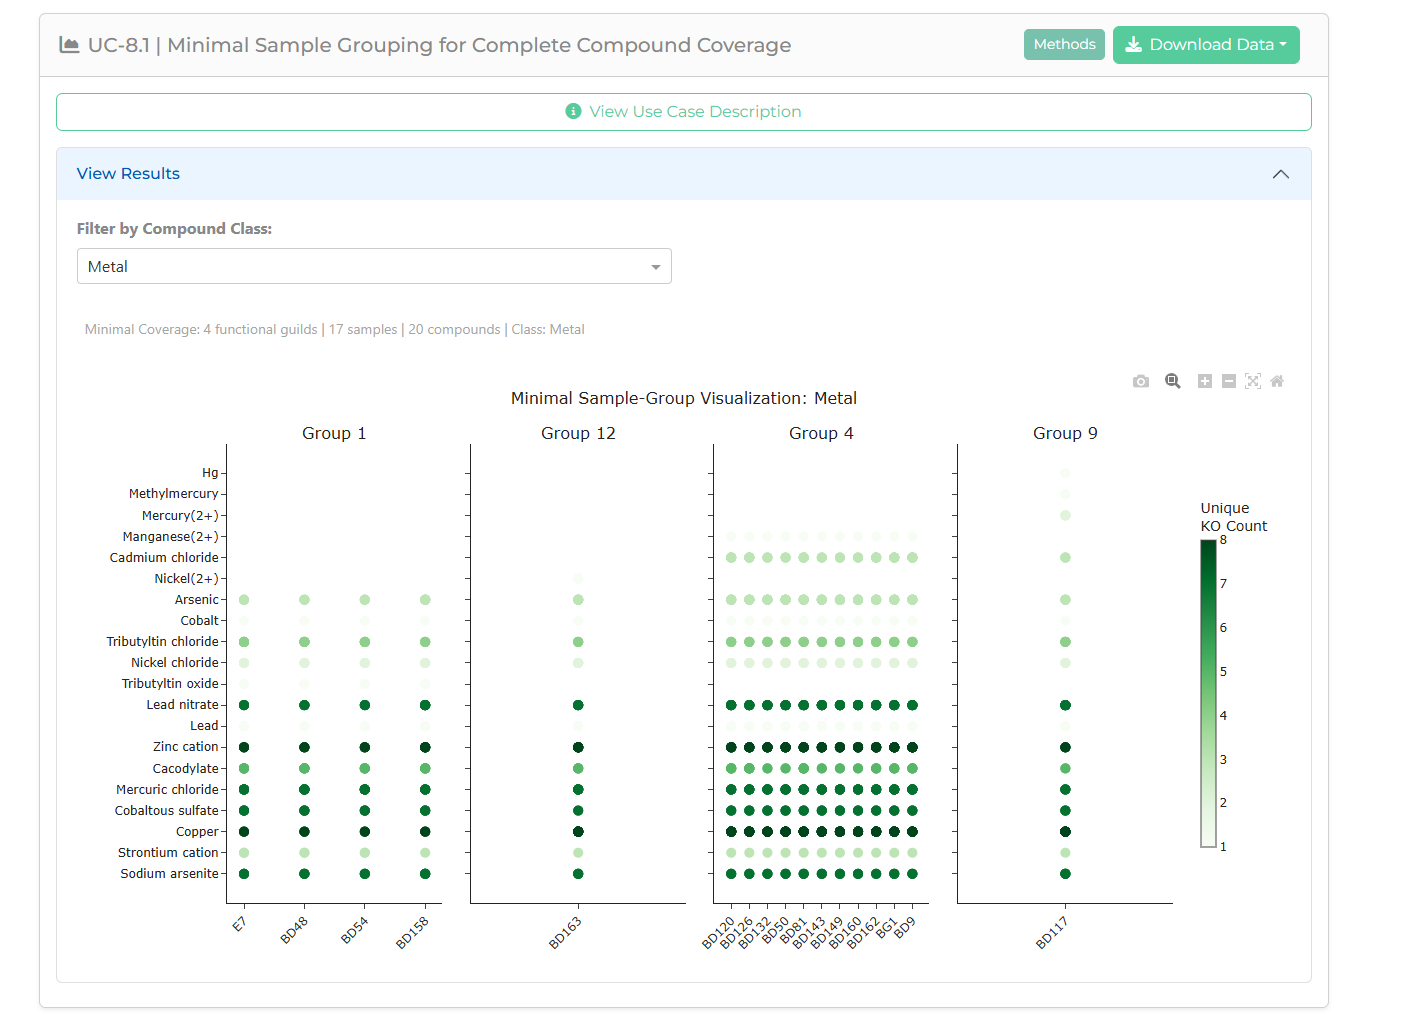
\includegraphics[width=0.95\textwidth]{UC_8.1/UC8.1_METAL.png}
    \caption{Agrupamento mínimo de amostras para cobertura de compostos da classe Metal.}
    \label{fig:metal}
\end{figure}

Esse filtro produziu um conjunto de isolados candidatos que foram posteriormente reavaliados quanto à cobertura de compostos alifáticos e poliaromáticos. Assim, a resistência a metais funcionou como um critério anterior de elegibilidade e consistência ambiental, enquanto a escolha final de cada consórcio foi guiada pela cobertura de hidrocarbonetos e pelo suporte experimental.

\section{Metodologia}

Para cada classe-alvo, os isolados foram comparados por perfis de cobertura de compostos. Isolados com perfis equivalentes foram tratados como membros de uma mesma guilda funcional. A seleção buscou representar as guildas necessárias com uma composição experimental compacta, evitando que o consórcio fosse definido principalmente pelo isolado de maior inventário.

Na refatoração final, os isolados de maior contribuição isolada foram removidos da composição experimental para reduzir redundância e tornar o teste mais interpretável. Assim, \textbf{BD163} foi removido do consórcio alifático e \textbf{BD61} foi removido do consórcio poliaromático. Ambos permanecem relevantes como referências de alta cobertura, mas não entram na composição final proposta.

Quando uma guilda tinha mais de um candidato funcionalmente equivalente, o DCPIP foi usado como critério experimental de desempate. Para compostos alifáticos, a métrica mais relevante foi a média de petróleo leve (\texttt{PL\_mean}). Para compostos poliaromáticos, a métrica mais relevante foi a média de petróleo pesado (\texttt{PP\_mean}). A média geral (\texttt{overall\_mean}) foi usada como suporte adicional.

As principais métricas usadas foram:

\begin{itemize}
    \item número de compostos cobertos pela combinação de isolados;
    \item contribuição individual de compostos por representante no trio final;
    \item completude de KOs por classe;
    \item desempenho DCPIP em petróleo leve e pesado;
    \item inventário gênico e interseções de KOs entre os membros;
    \item amplitude e profundidade de mitigação de risco.
\end{itemize}

\section{Consórcio orientado a compostos alifáticos}

O consórcio alifático selecionado foi composto por \textbf{BD127}, \textbf{E7} e \textbf{BD117}. Após a remoção do isolado dominante da modelagem inicial, essa combinação cobre \textbf{52 de 59 compostos alifáticos}, correspondendo a \textbf{88,14\%} de cobertura anotacional.

\begin{figure}[H]
    \centering
    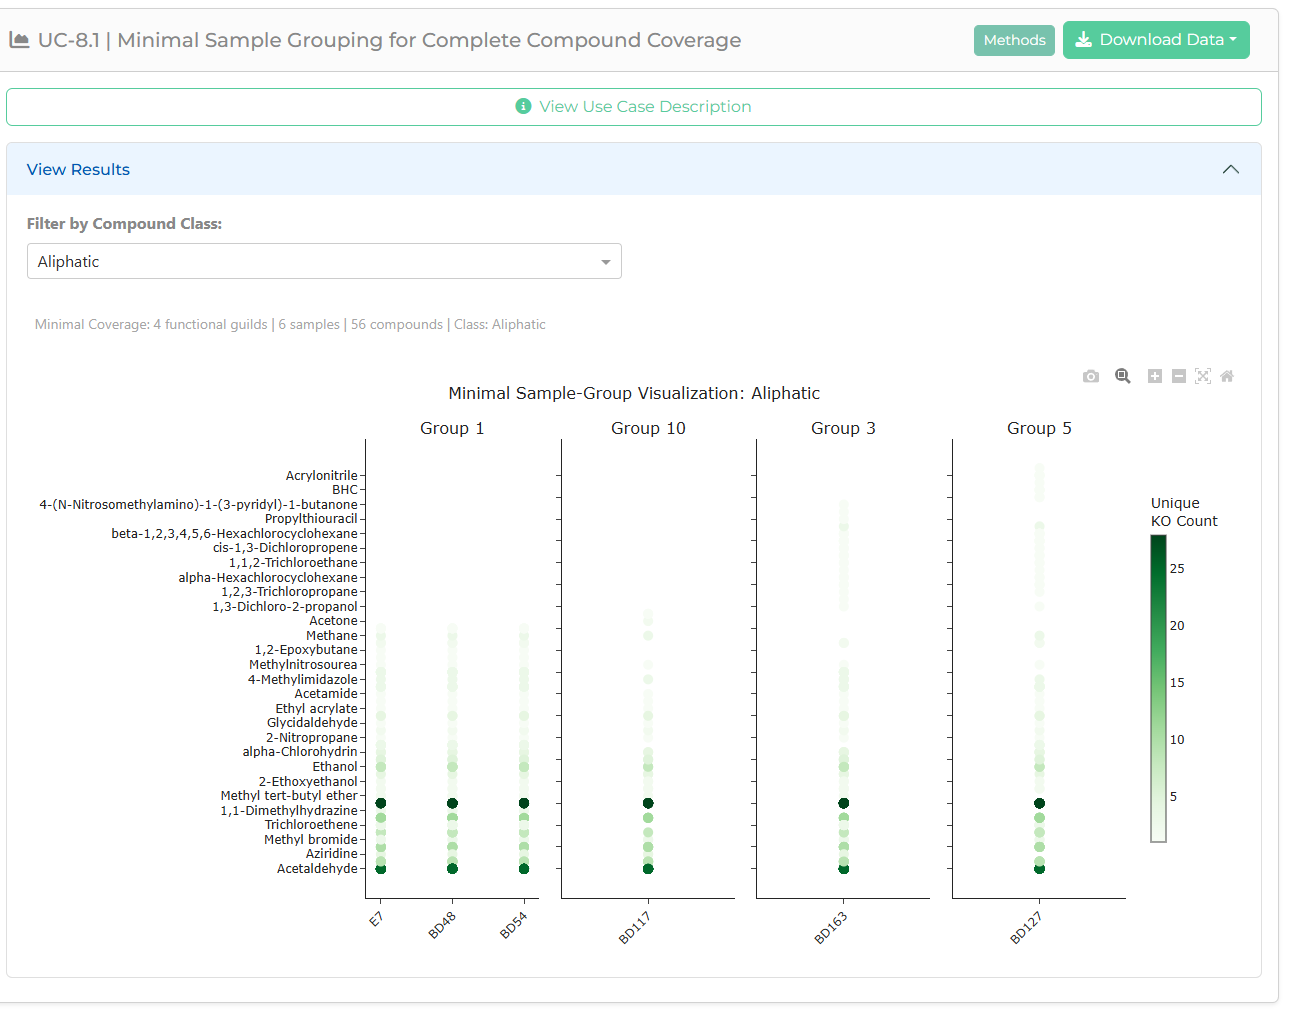
\includegraphics[width=0.95\textwidth]{UC_8.1/UC8.1_ALIPHATIC.png}
    \caption{Agrupamento mínimo de amostras para cobertura de compostos alifáticos dentro do universo elegível.}
    \label{fig:aliphatic}
\end{figure}

\begin{longtable}{p{1.6cm}p{2.8cm}p{2.0cm}p{1.8cm}p{2.0cm}p{4.2cm}}
\caption{Contribuição dos isolados no consórcio alifático.}\\
\toprule
\textbf{Isolado} & \textbf{Táxon} & \textbf{Compostos do isolado} & \textbf{PL médio} & \textbf{KO completo} & \textbf{Contribuição} \\
\midrule
\endfirsthead

\toprule
\textbf{Isolado} & \textbf{Táxon} & \textbf{Compostos do isolado} & \textbf{PL médio} & \textbf{KO completo} & \textbf{Contribuição} \\
\midrule
\endhead

BD127 & \textit{Achromobacter} & 43 & 59,21 & 36,60\% & Sustenta a maior fração de cobertura do trio sem manter o isolado dominante original. \\
E7 & \textit{Acinetobacter} & 34 & 82,91 & 39,22\% & Mantém forte desempenho em DCPIP para petróleo leve e acrescenta complementaridade funcional. \\
BD117 & \textit{Micococcus luteus} & 27 & 79,18 & 25,49\% & Contribui como membro complementar, com alto DCPIP e cobertura de compostos residuais. \\
\bottomrule
\end{longtable}

Na guilda formada por \textbf{E7}, \textbf{BD48} e \textbf{BD54}, com cobertura equivalente, \textbf{E7} foi mantido pelo maior \texttt{PL\_mean} (\textbf{82,91}), adotado como critério prioritário para o consórcio alifático. A cobertura do trio é menor que a da modelagem inicial com quatro membros, mas o desenho fica menos dependente de um único isolado de alta contagem e mais adequado para validação experimental.

\section{Consórcio orientado a compostos poliaromáticos}

O consórcio poliaromático selecionado foi composto por \textbf{BD120}, \textbf{BD158} e \textbf{BD117}. Após a remoção do isolado dominante da modelagem inicial, essa combinação cobre \textbf{35 de 44 compostos poliaromáticos}, correspondendo a \textbf{79,55\%} de cobertura.

\begin{figure}[H]
    \centering
    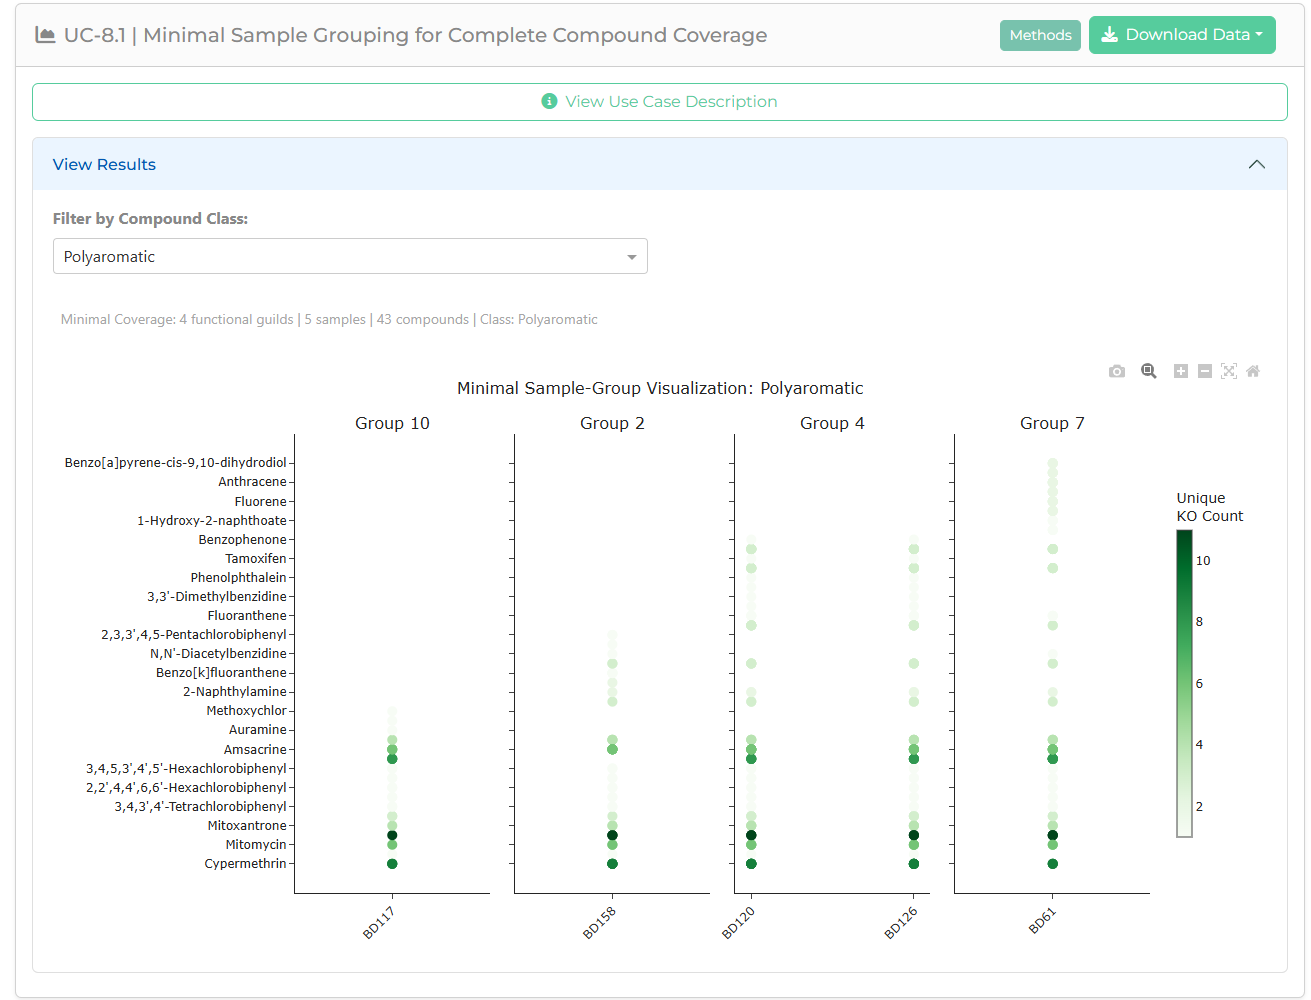
\includegraphics[width=0.95\textwidth]{UC_8.1/UC8.1_POLYAROMATIC.png}
    \caption{Agrupamento mínimo de amostras para cobertura de compostos poliaromáticos dentro do universo elegível.}
    \label{fig:polyaromatic}
\end{figure}

\begin{longtable}{p{1.6cm}p{2.8cm}p{2.0cm}p{1.8cm}p{2.0cm}p{4.2cm}}
\caption{Contribuição dos isolados no consórcio poliaromático.}\\
\toprule
\textbf{Isolado} & \textbf{Táxon} & \textbf{Compostos do isolado} & \textbf{PP médio} & \textbf{KO completo} & \textbf{Contribuição} \\
\midrule
\endfirsthead

\toprule
\textbf{Isolado} & \textbf{Táxon} & \textbf{Compostos do isolado} & \textbf{PP médio} & \textbf{KO completo} & \textbf{Contribuição} \\
\midrule
\endhead

BD120 & \textit{Bacillus subtilis} & 27 & 81,81 & 48,19\% & Sustenta a maior resposta experimental em petróleo pesado e boa completude KO. \\
BD158 & \textit{Salinicola} & 21 & 58,54 & 37,35\% & Mantém cobertura complementar e repertório funcional adicional. \\
BD117 & \textit{Micococcus luteus} & 17 & 76,65 & 22,89\% & Atua como membro complementar com alto DCPIP e compostos residuais. \\
\bottomrule
\end{longtable}

Na guilda formada por \textbf{BD120} e \textbf{BD126}, com função equivalente, \textbf{BD120} foi mantido pelo maior desempenho experimental, com \texttt{PP\_mean} de \textbf{81,81} e \texttt{overall\_mean} de \textbf{82,89}, frente a \textbf{39,05} e \textbf{49,66} para \textbf{BD126}. A retirada de \textbf{BD61} reduz a cobertura total, mas remove o isolado de maior contribuição isolada e permite testar um consórcio poliaromático menos dominado por um único membro.



\section{Consórcio controle negativo}

Para avaliar a associação entre menor repertório genômico e menor potencial de degradação, foi definido o controle negativo \textbf{BD2 + BD161}, aplicável aos ensaios alifáticos e poliaromáticos.

\begin{table}[H]
\centering
\small
\caption{Composição proposta para o consórcio controle negativo.}
\begin{tabular}{llccccc}
\toprule
\textbf{Isolado} & \textbf{Táxon} & \textbf{Genes alif.} & \textbf{Genes arom.} & \textbf{PL médio} & \textbf{PP médio} & \textbf{Média geral} \\
\midrule
BD2 & \textit{Staphylococcus} & 35 & 23 & 28,31 & 11,99 & 22,87 \\
BD161 & \textit{Rossellomorea} & 50 & 33 & 32,67 & 47,57 & 40,12 \\
\bottomrule
\end{tabular}
\normalsize
\end{table}

\textbf{BD2} foi priorizado como controle negativo por combinar menor repertório gênico para as classes alifática e aromática com baixo desempenho em DCPIP. \textbf{BD161} complementa o controle por apresentar baixo \texttt{PL\_mean} e repertório gênico reduzido.

Assim, o controle negativo foi definido pela combinação de menor suporte anotacional e menor resposta experimental.

\section{Resumo}


\begin{itemize}
    \item \textbf{BD127 + E7 + BD117}: consórcio alifático de três membros, com cobertura anotacional relevante e suporte experimental em petróleo leve.
    \item \textbf{BD120 + BD158 + BD117}: consórcio poliaromático de três membros, com composição menos redundante e suporte experimental em petróleo pesado.
    \item \textbf{BD2 + BD161}: controle negativo, definido por menor suporte genômico e menor resposta em DCPIP.
\end{itemize}

A seleção integrou cobertura de compostos, complementaridade funcional e desempenho em DCPIP, utilizando as análises de casos de uso complementares do BioRempp como suporte ao repertório gênico e enzimático dos isolados.

\end{document}
